% 9. előadás vége, 10. előadás

\chapter{Szál szinten párhuzamos architektúrák}

\section{Bevezetés}
Az Intel 80386-os processzora óta bevezetett újítások a fogyasztás és a lapkaméret növekedésével jártak, viszont ehhez képest a teljesítmény csak kisebb mértékben javult.
Tehát a teljesítmény növekedése nem állt egyenes arányban a komplexitás növekedésével.
Ez elsősorban az egy magos processzorokra igaz.
Következmény, hogy egyre több tranzisztor kell és nő a fogyasztás.
Ennek megoldásához el kellett térni a klasszikus tervezési elvektől, ahol csak utasítás szinten használták ki a párhuzamosságokat.
A fejlődés következő lépcsőjét a szál szintű párhuzamosság kihasználása jelentette.

\section{A szál}
A szál a program legkisebb önállóan végrehajtható része $\rightarrow$ párhuzamosan futtatható.
Míg az utasítás szintű párhuzamosság felderítésére önmagában képes a hardver, a szálak kihasználásához az operációs rendszer támogatására is szükség van.
A párhuzamosság lehet
\begin{itemize}
    \item implicit: a programozó szekvenciális programot ír, a hardver és a szoftver párhuzamosítja a kódot,
    \item explicit: a programozó kifejezetten párhuzamos programot ír.
\end{itemize}
Fontos, hogy egy szálon belül nincs párhuzamosság, ezért a teljesítmény növeléséhez több szál létrehozása szükséges.
Ez egy magasabb szintű párhuzamosság, így összetettebb is.

\subsection{Szálak származtatása}
\begin{itemize}
    \item Különböző alkalmazásokból (multiprogramozás).
    \item Ugyanabból az alkalmazásból:
    \begin{itemize}
        \item multitasking
        \item multithreading
    \end{itemize}
\end{itemize}

\subsection{Többszálúság csoportosítása}
\begin{itemize}
    \item Szoftveres: többszálú alkalmazás futtatása egyszálú CPU-n, pl. időosztással.
    \item Hardveres: többszálú alkalmazás futtatása többszálú CPU-n. Többszálú processzorok:
    \begin{itemize}
        \item SMP - Symmetric MultiProcessing (\ref{fig:smp}. ábra).
        \item SMT - Simultaneous MultiThreading (\ref{fig:smt}. ábra). Kb. 5\% komplexitás növekedéssel 0-30\%-os teljesítmény növekedés érhető el a segítségével.
    \end{itemize}
\end{itemize}

\begin{figure}[H]
    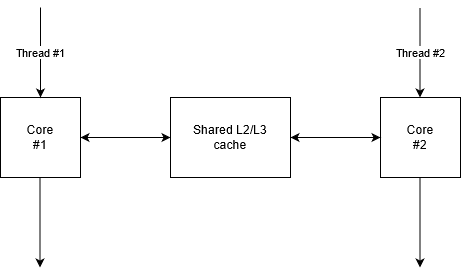
\includegraphics[width=0.6\textwidth]{smp}
    \centering
    \caption{SMP CPU}
    \label{fig:smp}
\end{figure}
\begin{figure}[H]
    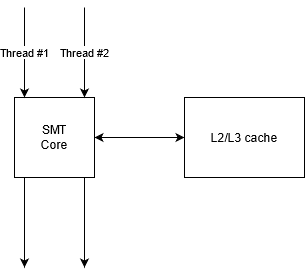
\includegraphics[width=0.4\textwidth]{smt}
    \centering
    \caption{SMT CPU}
    \label{fig:smt}
\end{figure}

\section{Több szál futtatása P4 CPU-n (Hyper Threading nélkül)}
A futószalag bonyolult, sok fokozatú, ezért sok függőség lép fel.
A függőségek miatt egy feladat befejezése előtt gyakran szükséges egy másik elkezdése, azonban egy új szál futtatásánál az aktív szál kontextusának mentésével kell kezdeni.
Ezután a másik szál kontextusát be kell tölteni és folytatni a végrehajtást.
A kontextus váltás akár 2-3 ezer óraciklus is lehet, tehát nagyon erőforrás igényes.
A multimédiás alkalmazások és a több alkalmazást futtató felhasználó miatt még gyakrabban volt szükség kontextus váltásra.
A kontextus váltások csökkentése miatt jelentek meg a többszálú architektúrák.

\section{Operációs rendszerek szálkezelése}
A modern operációs rendszerek minden folyamatra külön lap táblát tartanak nyilván, ez a TLB (Translation Lookaside Buffer).
Ezekben tárolódik az adott folyamat kontextusa, ami a memóriában vagy a háttértáron tárolódik.
Tehát a szálkezelés hardveres és szoftveres támogatás is igényel.

\section{Szál szinten párhuzamos architektúrák osztályozása}

\subsection{Finoman szemcsézett}
A CPU 2 vagy több szálat futtat, órajelenként vált a szálak között.
A gyakori kontextus váltások miatt az ilyen processzorok több regisztert tartalmaznak, így azokban több szál adatai is elférnek (nem kell várni a memóriából betöltésre).
Pl. két szálú CPU esetén mindkét szál kontextusát tároljuk a regiszterekben és egy kontextus kapcsoló segítségével történik a váltás.
Következmény, hogy nincs késleltetés a váltások között.
A teljesítmény növekszik, pl. ha az egyik szál valamilyen függőségre vár, az nem blokkolja a másik szálat (cél az üresjáratok feltöltése).
0-20\%-os teljesítmény növekedést eredményezhet.

\subsection{Eseményvezérelt (SoEMT - Switch on Event MultiThreading)}
Amennyiben az egyik szál futása megakad (pl. függőség miatt), akkor vált a másikra.
Probléma, hogy a szál megakadását érzékelni kell, ami általában 1-2 óraciklus időigényű.

\subsection{SMT (Simultaneous MultiThreading)}
Az elvét 1968-ban írták le, gyakorlati megvalósítása viszont csak a 2000-es években kezdődött el.
Ennek egyik gyakorlati megvalósítása az Intel Hyper Threading.
Lényege, hogy az összes szál futtatása párhuzamosan történik.
\subsubsection{Hardveres megvalósítás}
Az SMT-t támogató processzorok elsősorban szuperskalár architektúrák. A párhuzamosság megvalósításához az alábbi harveres követelményeknek kell megfelelniük:
\begin{itemize}
    \item Számos erőforrást meg kell többszörözni (pl. szálankénti program counter, regiszter tároló).
    \item Az erőforrásokat meg kell tudni osztani a szálak között (szükség esetén egyesíteni is, hogy egy szál megakadása esetén az aktív szál a teljes processzort tudja használni).
\end{itemize}

\section{Az Intel Hyper Threading}
Az Intel Hyper Threading technológia egy két szálas SMT architektúra.
Először a Northwood alapú Pentium 4-es processzorokba került be.
A két szál utasításait egyszerre hajtja végre, out of order kiküldéssel.
Egy mag az operációs rendszer számára két külön logikai magnak látszódik, ezért úgy ütemezi az utasításokat, mintha két processzoros rendszeren futna.
Tehát egy CPU egyszerre két logikai CPU utasításait hajtja végre.
A processzorban ekkor egyszerre két architekturális állapot van jelen.

\subsection{Üzemmódok}
\subsubsection{ST (single task)}
Egy szál végrehajtása történik, a megosztott erőforrások egyesítésre kerülnek.
Két állapota lehet, attól függően, hogy melyik logikai CPU aktív:
\begin{itemize}
    \item ST0
    \item ST1
\end{itemize}
\subsubsection{MT (multi task)}
Több szál végrehajtása történik párhuzamosan.
\subsubsection{Váltás}
A processzor először MT módban indul.
Ha az egyik szál megakad, ST módba vált a processzor.
A függőség megszűnésével a CPU visszakerül MT üzemmódba.
Az üzemmódok közötti váltás a HALT utasítás segítségével történik, ami megszakítja a CPU futását és energiatakarékos állapotba helyezi.
Ezt csak az OS, vagy más, alacsony szintű alkalmazás adhatja ki.

\subsection{Működési vázlat (Intel Pentium 4 HT)}
\begin{figure}[H]
    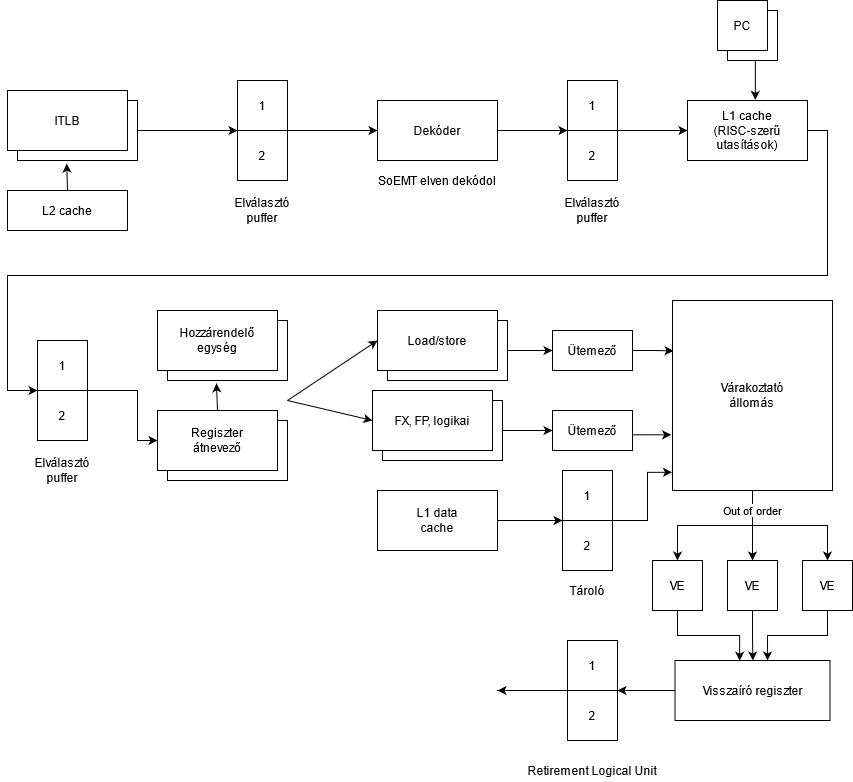
\includegraphics[width=\textwidth]{ht}
    \centering
    \caption{Az Intel Hyper Threading működése}
    \label{fig:ht}
\end{figure}

\section{Az SMT megvalósítási céljai}
\begin{itemize}
    \item Kis magméret növekedés.
    \item Egy szál várakozása esetén a másik szál gond nélkül futhasson, folytathassa a műveletek végrehajtását.
    \item Egy szál futása esetén a végrehajtás ugyanolyan gyors legyen, mint egy egy szálas CPU-n.
\end{itemize}